\documentclass[12pt]{article}

\usepackage{sbc-template}
\usepackage[utf8]{inputenc}
\usepackage[brazil]{babel}
\usepackage{graphicx}
\usepackage{booktabs}
\usepackage{url}

\sloppy

\title{Recuperação da Informação para RAG Educacional: avaliação de BM25, busca densa e fusão híbrida}

\author{Fabiana Marques Costa\inst{1}, Marcos Hideki Nishida Sakaguchi\inst{1}}

\address{Programa de Pós-Graduação em Ciência da Computação -- Instituto de Geociências e Ciências Exatas\\
Universidade Estadual Paulista Júlio de Mesquita Filho (UNESP)\\
Rio Claro -- SP -- Brasil
\email{fabiana.m.costa@unesp.br, marcos.sakaguchi@unesp.br}
}

\begin{document}

\maketitle

\begin{abstract}
Retrieval quality constrains the evidence available to Retrieval-Augmented
Generation (RAG) tutors. This paper evaluates BM25, dense retrieval with
BGE-M3, and hybrid retrieval by Reciprocal Rank Fusion in three reproducible
retrieval studies: SciQ (878 test queries and 12,135 indexed support passages),
a 49-page educational PDF, and a 581-page Information Retrieval textbook. The
two PDF collections contain 50 evidence-anchored development queries each. The
hybrid method achieved the highest MRR@10 and Recall@10 in SciQ (0.797 and
0.968) and in the 49-page collection (0.815 and 0.970). In the textbook,
dense and hybrid retrieval outperformed BM25; the hybrid method reached 0.709
MRR@10 and 0.960 Recall@10, against 0.576 and 0.810 for BM25. Source-level
evidence is materialized into chunk identifiers for each segmentation strategy,
which supports a separate chunking ablation. The results concern retrieval;
evaluation of generated RAG answers is left for future work.
\end{abstract}

\begin{resumo}
A qualidade da recuperação limita as evidências disponíveis para tutores
baseados em \textit{Retrieval-Augmented Generation} (RAG). Este artigo avalia
BM25, recuperação densa com BGE-M3 e recuperação híbrida por \textit{Reciprocal
Rank Fusion} em três estudos reproduzíveis de RI: SciQ (878 consultas de teste
e 12.135 parágrafos de suporte indexados), um PDF educacional de 49 páginas e
um livro de Recuperação da Informação de 581 páginas. As duas coleções em PDF
contêm 50 consultas de desenvolvimento ancoradas em evidências. O método
híbrido obteve os maiores MRR@10 e Recall@10 no SciQ (0,797 e 0,968) e na
coleção de 49 páginas (0,815 e 0,970). No livro de RI, os métodos denso e
híbrido superaram o BM25; o híbrido atingiu MRR@10 de 0,709 e Recall@10 de
0,960, ante 0,576 e 0,810 do BM25. A evidência é registrada no documento-fonte
e materializada em identificadores de \textit{chunks} para cada segmentação,
permitindo uma ablação específica de \textit{chunking}. Os resultados tratam
da recuperação; a avaliação das respostas geradas pelo RAG permanece como
trabalho futuro.
\end{resumo}

\section{Introdução}

Modelos de linguagem ampliam as possibilidades de diálogo e explicação em
Sistemas Tutores Inteligentes (ITS), mas a fluência da resposta não assegura
correção, rastreabilidade ou aderência ao material da disciplina
\cite{woolf2009,kuhail2023}. RAG busca reduzir esse problema ao condicionar a
geração a evidências recuperadas de uma base documental \cite{lewis2020}. Em
um tutor, porém, a resposta só pode ser tão bem fundamentada quanto os trechos
que o recuperador disponibiliza ao modelo gerador.

Este trabalho trata a Recuperação da Informação (RI) como objeto experimental
principal. Comparamos BM25, recuperação densa e fusão híbrida em um benchmark
controlado e em dois corpora educacionais em PDF. As contribuições são: (i) um
protocolo que preserva a evidência no documento-fonte antes de derivar os
\textit{chunks}; (ii) resultados atualizados e rastreáveis em três conjuntos;
e (iii) uma ablação de segmentação separada da comparação entre recuperadores.
Não são reportadas métricas de respostas geradas: essa camada será executada
somente após a consolidação de um conjunto independente de avaliação.

\section{Recuperação e Avaliação em RAG Educacional}

BM25 é uma referência eficiente para correspondência lexical, particularmente
quando termos técnicos da consulta ocorrem no material \cite{manning2008,
robertson2009}. A recuperação densa representa consultas e passagens em um
espaço vetorial e pode atender melhor a paráfrases ou vocabulários distintos
\cite{karpukhin2020}. A estratégia híbrida combina as listas dos dois
recuperadores; neste estudo, a combinação é feita por \textit{Reciprocal Rank
Fusion} (RRF) \cite{cormack2009}.

Avaliar apenas a resposta final esconderia se um erro decorre da recuperação ou
da geração. Por isso, a primeira camada do protocolo mede o ranqueamento com
MRR, MAP, nDCG, Recall e Hit Rate. Métricas de fidelidade e relevância de
resposta, como as propostas pelo RAGAS \cite{ragas2023}, ficam para a etapa
posterior de geração. Essa separação é particularmente importante em RAG,
pois a qualidade de documentos recuperados e a utilidade para a geração não
são necessariamente equivalentes \cite{salemi2024}.

\section{Método}

\subsection{Conjuntos e julgamentos de relevância}

O SciQ \cite{sciq2017} fornece uma baseline controlada: cada uma das 878
consultas do conjunto de teste possui um único parágrafo de suporte relevante,
entre 12.135 passagens indexadas. Os outros dois conjuntos são de
desenvolvimento e foram construídos para validar a instrumentação em materiais
educacionais reais: \textit{A importância do ato de ler}, de Paulo Freire
\cite{freire1989}, com 49 páginas, 50 consultas e 69 evidências; e
\textit{Introduction to Information Retrieval}, com 581 páginas, 50 consultas
e 107 evidências \cite{manning2008}.

Em ambos os PDFs, cada caso registra o hash do arquivo, a página, a citação e
o grau de relevância da evidência. Esse registro é materializado nos
identificadores de \textit{chunks} de cada condição, evitando que uma mudança
de segmentação invalide os julgamentos. As 69 e 107 evidências, respectivamente,
foram localizadas e materializadas integralmente nas rodadas reportadas. Os
casos de PDF foram redigidos com apoio de IA e revisados por um único anotador;
portanto, são tratados como desenvolvimento, e não como teste independente.

\subsection{Condições e métricas}

Todos os métodos usam a mesma coleção por corpus e a segmentação
\texttt{recursive\_text} na comparação principal. BM25 fornece a busca
esparsa; a busca densa usa BGE-M3; e o híbrido aplica RRF aos dois rankings.
As consultas recebem até dez passagens. Reportamos MRR@10, MAP@10, nDCG@10,
Recall@10 e Hit@10. No SciQ, como há uma única evidência por pergunta,
Recall@k equivale a Hit@k e MAP@k coincide com MRR@k.

Os intervalos de confiança de 95\% foram estimados por \textit{bootstrap}
pareado com 2.000 reamostragens. Para Hit@10, as comparações entre métodos usam
o teste exato de McNemar com correção de Holm. Cada rodada preserva manifesto,
resultados por consulta, métricas, gráficos e versões de dependências.

\section{Resultados de Recuperação}

A Tabela~\ref{tab:resultados} reúne os resultados no top-10. A Figura~\ref{fig:sciq-recall-k}
mostra como a cobertura no SciQ cresce com $k$, enquanto a
Figura~\ref{fig:resultados-tres-corpora} permite comparar descritivamente os
três conjuntos.

\begin{table*}[t]
\centering
\small
\caption{Resultados de recuperação no top-10. Valores maiores são melhores.}
\label{tab:resultados}
\begin{tabular}{llrrr}
\toprule
\textbf{Conjunto} & \textbf{Método} & \textbf{MRR@10} & \textbf{nDCG@10} & \textbf{Recall@10} \\
\midrule
SciQ & BM25 & 0,775 & 0,819 & 0,952 \\
SciQ & Denso & 0,719 & 0,769 & 0,923 \\
SciQ & Híbrido (RRF) & 0,797 & 0,839 & 0,968 \\
\midrule
\textit{Ato de Ler} & BM25 & 0,719 & 0,776 & 0,950 \\
\textit{Ato de Ler} & Denso & 0,703 & 0,762 & 0,960 \\
\textit{Ato de Ler} & Híbrido (RRF) & 0,815 & 0,848 & 0,970 \\
\midrule
Livro de RI & BM25 & 0,576 & 0,621 & 0,810 \\
Livro de RI & Denso & 0,708 & 0,745 & 0,940 \\
Livro de RI & Híbrido (RRF) & 0,709 & 0,754 & 0,960 \\
\bottomrule
\end{tabular}
\end{table*}

\subsection{SciQ}

O híbrido alcançou a maior cobertura em todos os valores de $k$: Hit@1 de
0,695 e Hit@10 de 0,968, contra 0,671 e 0,952 para BM25. No top-10, o ganho
de 0,016 em Hit Rate sobre BM25 foi significativo pelo teste de McNemar com
correção de Holm ($p=0{,}0066$); o ganho em MRR@10 foi 0,022, com IC95\%
pareado de $[0{,}0067; 0{,}0370]$. A recuperação densa ficou abaixo dos dois
demais métodos nesse benchmark. Assim, a fusão trouxe ganho mensurável sem
evidência de que apenas a similaridade semântica substitua a correspondência
lexical nesse cenário.

\begin{figure*}[t]
\centering
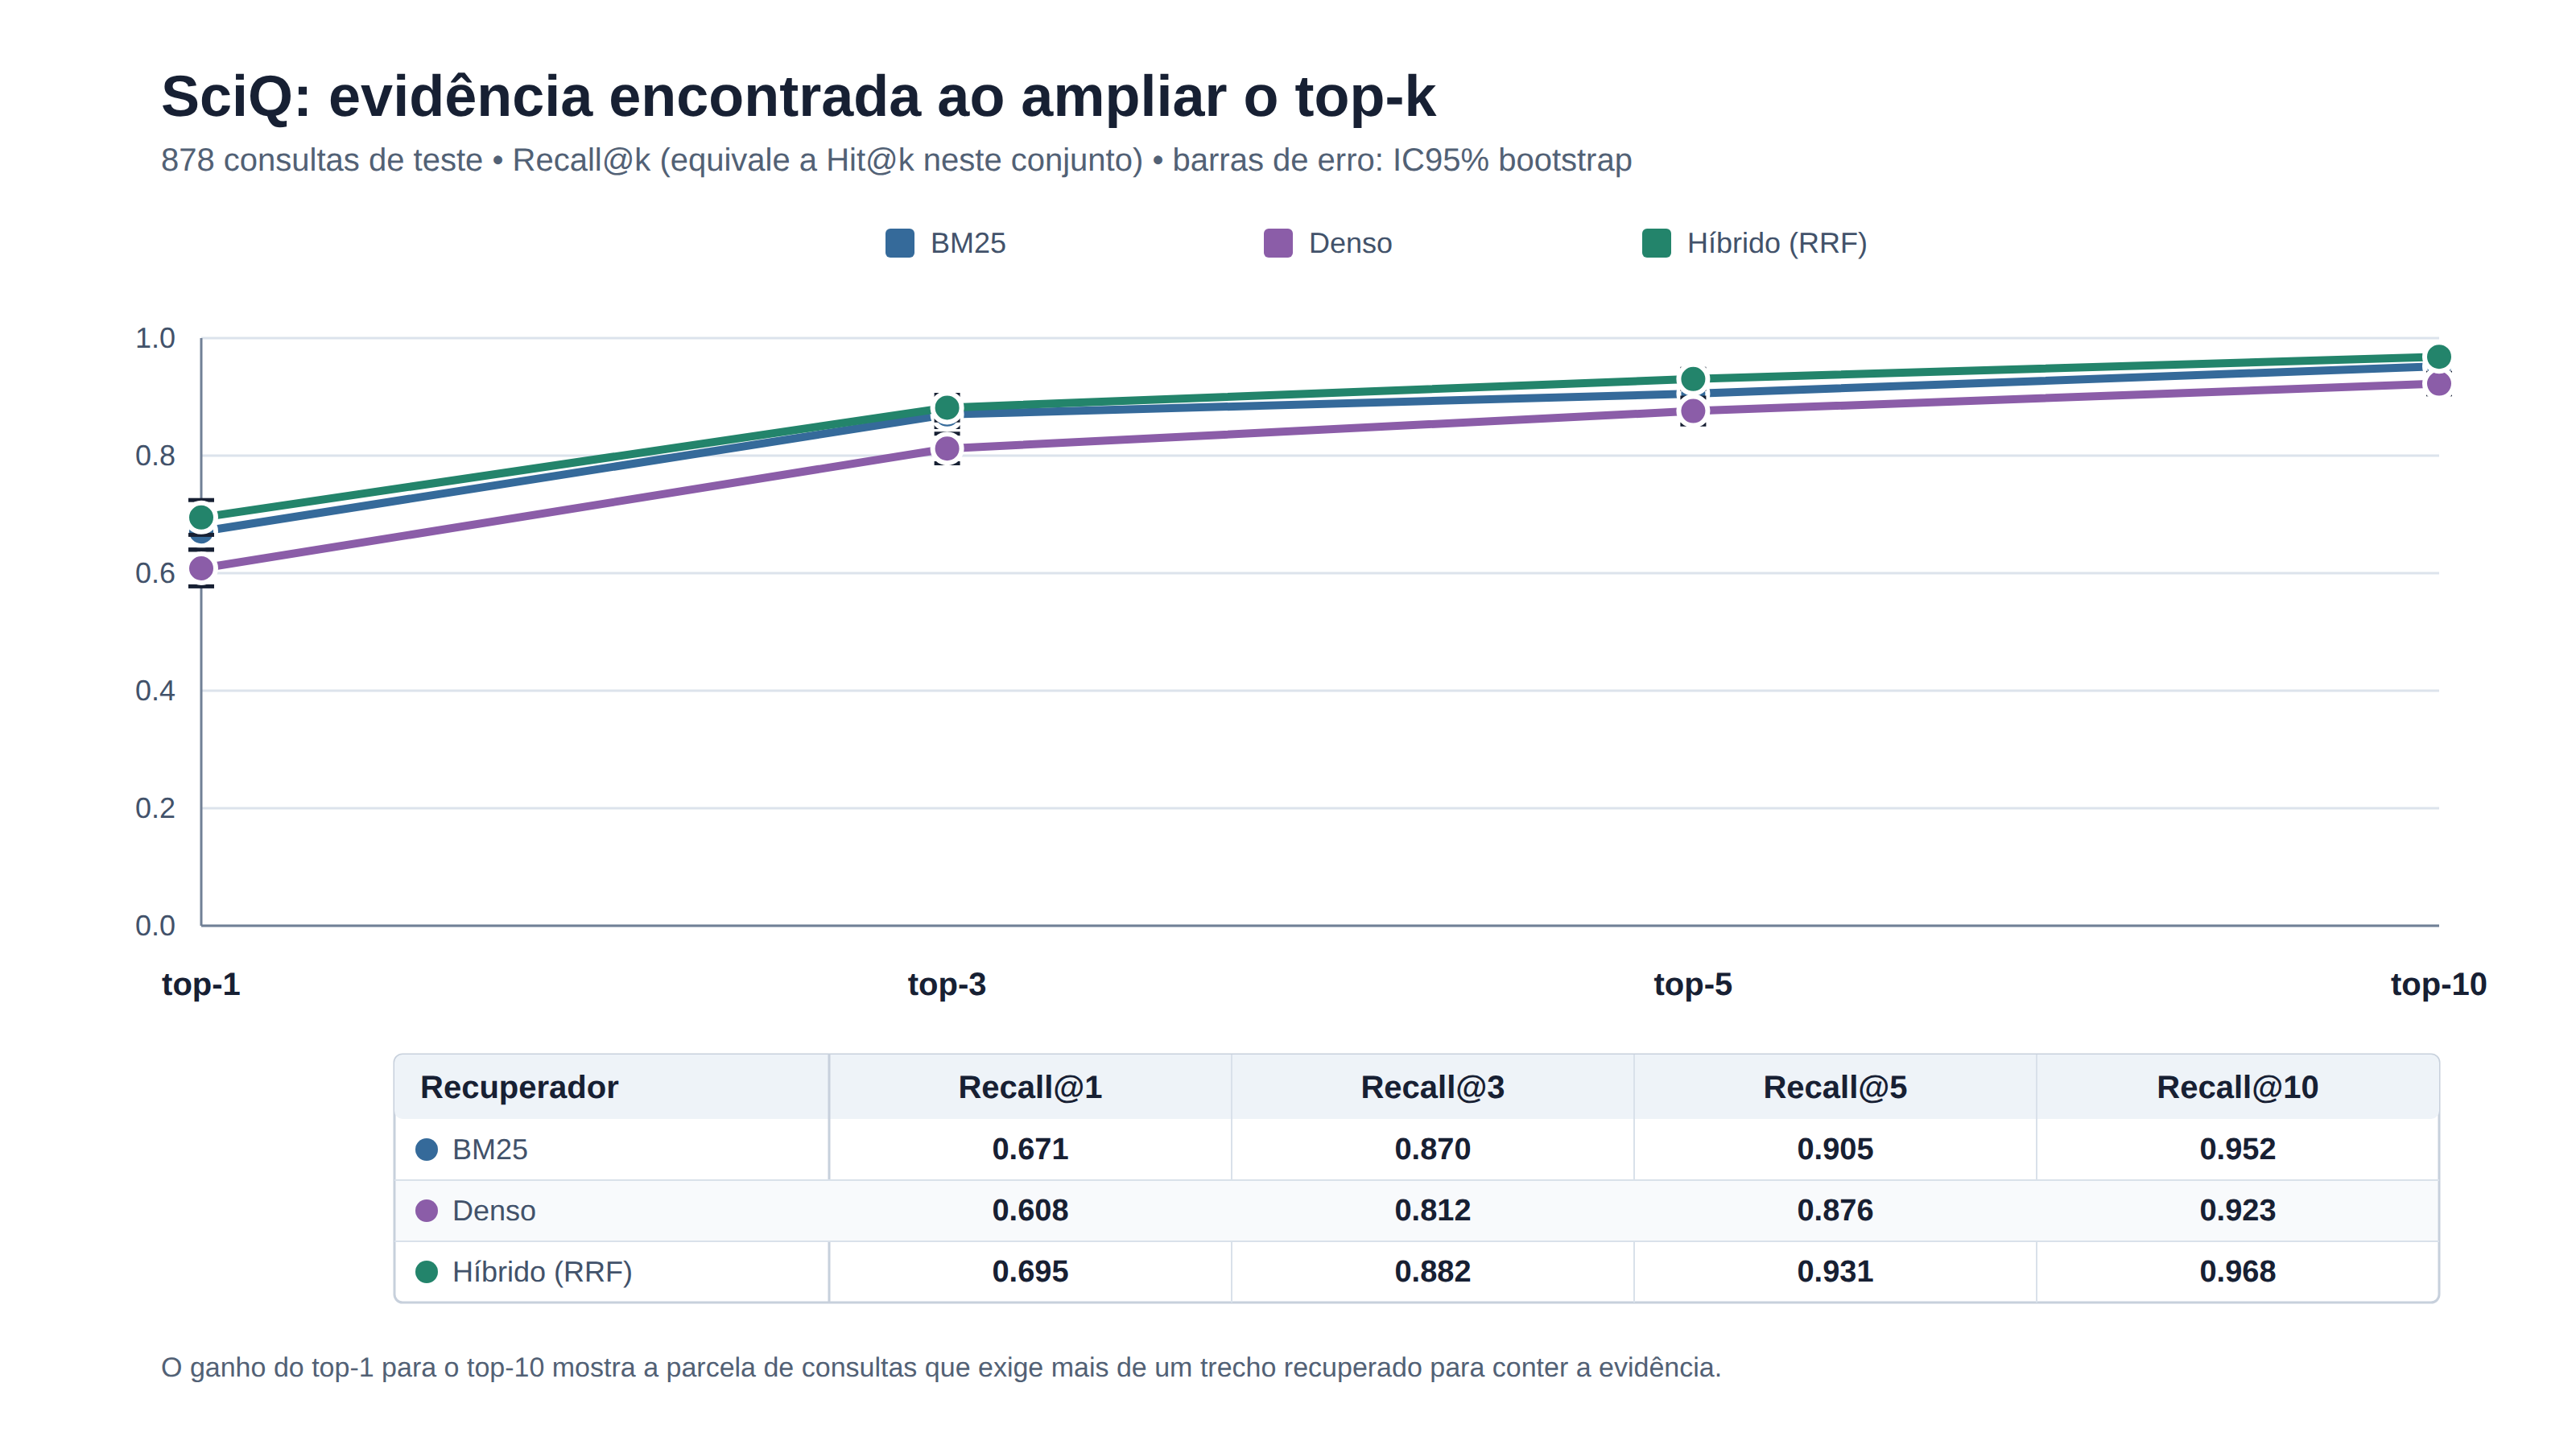
\includegraphics[width=0.98\textwidth]{../figures/slides_pdf_ir/05_sciq_recall_por_k.png}
\caption{Cobertura da evidência no SciQ ao variar $k$ (878 consultas de teste e
12.135 parágrafos de suporte indexados). As barras indicam IC95\% por
\textit{bootstrap}; como há uma única evidência relevante por consulta,
Recall@k equivale a Hit@k.}
\label{fig:sciq-recall-k}
\end{figure*}

\subsection{Corpora em PDF}

No \textit{Ato de Ler}, todos os métodos alcançaram cobertura alta no top-10,
mas o híbrido melhorou a qualidade do ranqueamento: MRR@10 de 0,815, frente a
0,719 (BM25) e 0,703 (denso). A diferença pareada de MRR entre híbrido e
BM25 foi 0,096, com IC95\% de $[0{,}021; 0{,}177]$. Esse resultado é
compatível com o uso complementar de sinais lexicais e semânticos em um corpus
educacional em português.

No livro de RI, as consultas estão em português, enquanto o texto indexado está
em inglês. Nessa condição cruzada, denso e híbrido atingiram Hit@10 de 0,980,
contra 0,820 do BM25 ($p_{\mathrm{Holm}}=0{,}0234$ em ambas as comparações).
Os valores de MRR@10 dos métodos denso e híbrido foram muito próximos (0,708 e
0,709), e o intervalo para sua diferença inclui zero. Logo, o resultado não
permite atribuir a vantagem ao tamanho do livro: tema, idioma e formulação das
consultas também mudam entre os dois PDFs.

\begin{figure*}[t]
\centering
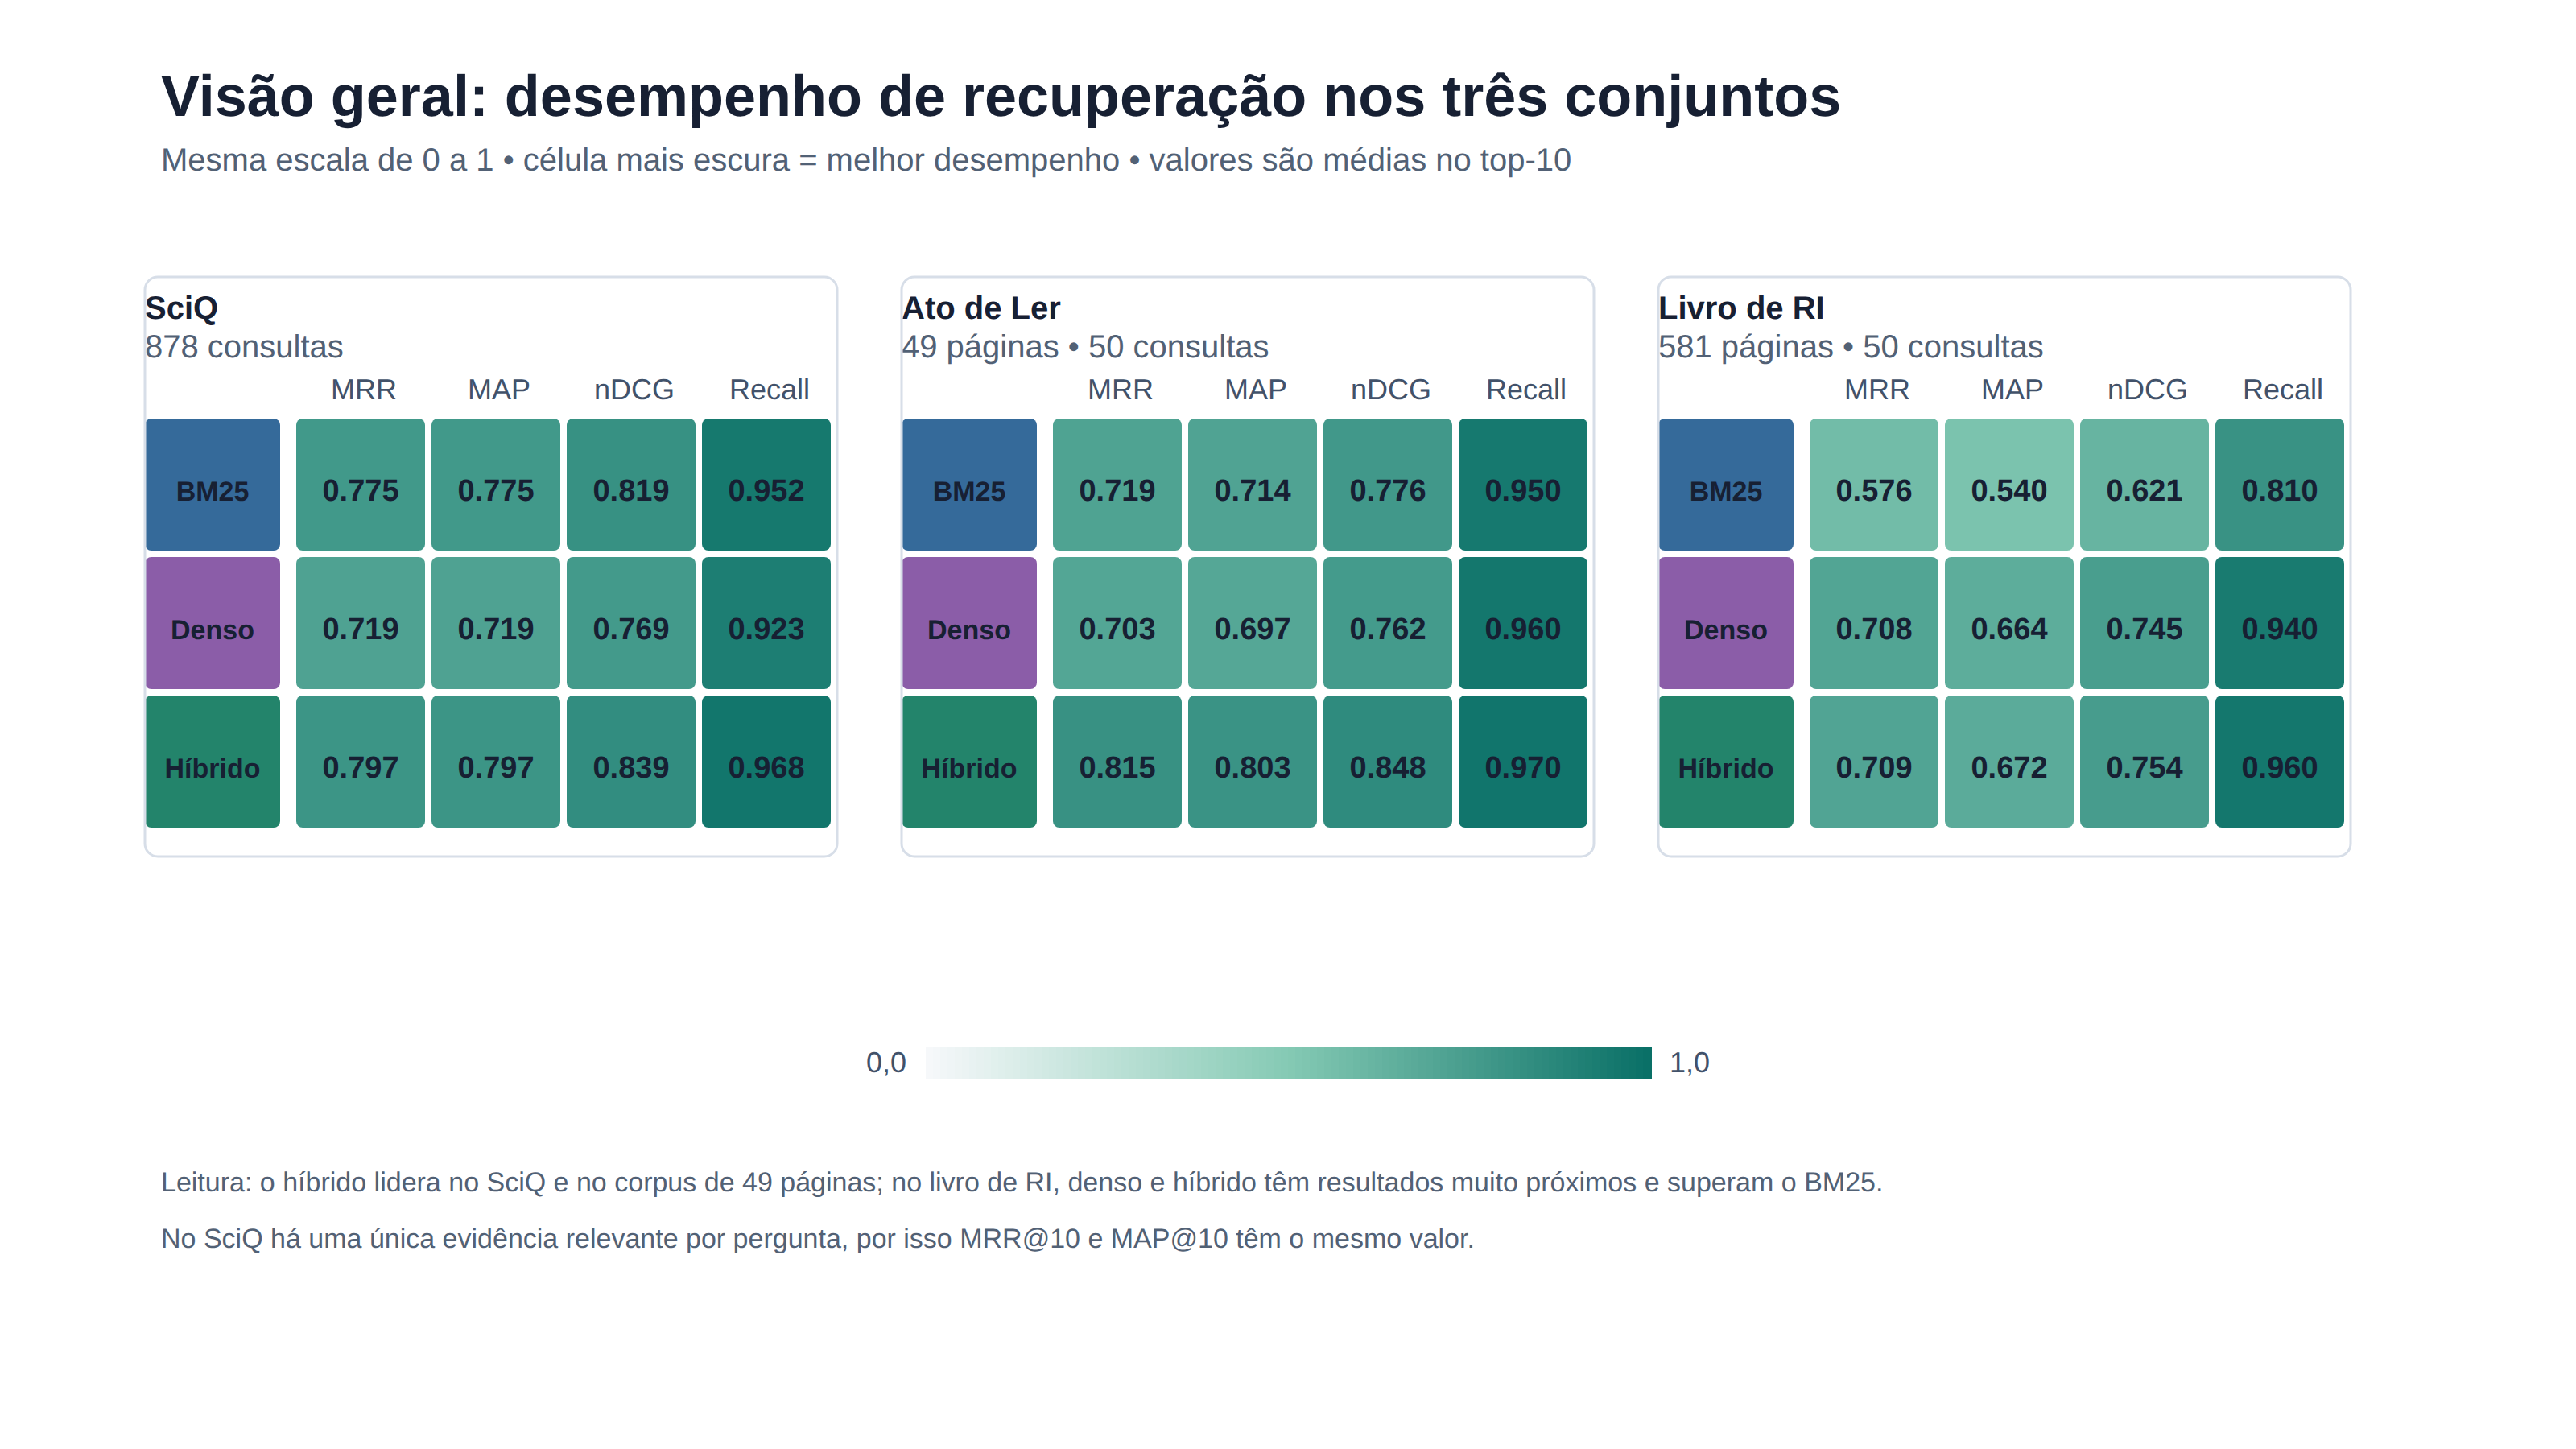
\includegraphics[width=0.98\textwidth]{../figures/slides_pdf_ir/07_heatmap_geral_tres_datasets.png}
\caption{Comparação descritiva do desempenho de recuperação no top-10 nos três
conjuntos avaliados. Valores maiores são melhores; no SciQ, MRR@10 e MAP@10
coincidem porque cada pergunta possui uma única evidência relevante.}
\label{fig:resultados-tres-corpora}
\end{figure*}

\subsection{Ablação de segmentação}

Mantendo o recuperador híbrido e as 50 consultas do \textit{Ato de Ler}, a
Tabela~\ref{tab:chunking} compara quatro estratégias de segmentação. Todas
materializaram as 69 evidências e obtiveram Hit@10 de 0,980. A segmentação
recursiva obteve o maior MRR@10 e nDCG@10, mas os intervalos de confiança se
sobrepõem; a ablação deve ser lida como evidência de robustez da instrumentação,
não como seleção definitiva de uma estratégia.

\begin{table}[t]
\centering
\small
\caption{Ablação de \textit{chunking} no \textit{Ato de Ler} com recuperação híbrida.}
\label{tab:chunking}
\begin{tabular}{lrrrr}
\toprule
\textbf{Estratégia} & \textbf{Chunks} & \textbf{MRR} & \textbf{nDCG} & \textbf{Recall} \\
\midrule
Fixa por tokens & 33 & 0,790 & 0,828 & 0,970 \\
Recursiva & 35 & 0,817 & 0,849 & 0,970 \\
Docling hierárquica & 395 & 0,794 & 0,823 & 0,960 \\
Docling híbrida & 70 & 0,802 & 0,842 & 0,980 \\
\bottomrule
\end{tabular}
\end{table}

\section{Limitações e Próximos Passos}

Os resultados em PDF ainda não estimam generalização: há 50 consultas por
coleção, perguntas apoiadas por IA e uma única revisão humana. Os julgamentos
ancorados em citações tornam a avaliação auditável, mas não eliminam a
incompletude de qrels nem substituem dupla anotação e adjudicação. As páginas
são metadados de auditoria: citações repetidas no mesmo documento podem
materializar mais de um qrel. O contraste entre os PDFs altera simultaneamente
domínio, idioma e consultas;
não pode ser interpretado como efeito isolado do tamanho do corpus. Os materiais
também exigem atenção a direitos autorais antes de sua distribuição como
benchmark.

O próximo passo é congelar um conjunto independente, com anotação humana por
mais de um avaliador, e reutilizá-lo na camada RAG. Nessa etapa, gerador,
prompt e $k$ serão mantidos constantes para relacionar as métricas de RI à
fidelidade, relevância e adequação pedagógica das respostas.

\section{Conclusão}

O estudo mostra que não há um recuperador universalmente melhor, mas que a
fusão híbrida foi a condição mais consistente nos conjuntos avaliados. Ela
liderou o SciQ e o \textit{Ato de Ler}; no livro de RI em condição
português--inglês, denso e híbrido superaram claramente o BM25 e permaneceram
próximos entre si. A separação entre comparação de recuperadores, materialização
de evidências e ablação de segmentação torna os resultados reproduzíveis e
evita atribuir à geração falhas que pertencem à recuperação. A avaliação das
respostas do tutor é a etapa necessária para verificar se esses ganhos se
traduzem em melhor apoio à aprendizagem.

\begin{thebibliography}{99}

\bibitem[Cormack et al. 2009]{cormack2009}
Cormack, G. V., Clarke, C. L. A. and Buettcher, S. (2009).
Reciprocal Rank Fusion Outperforms Condorcet and Individual Rank Learning
Methods. In \textit{Proceedings of the 32nd International ACM SIGIR
Conference on Research and Development in Information Retrieval}, p. 758--759.

\bibitem[Es et al. 2023]{ragas2023}
Es, S., James, J., Espinosa-Anke, L. and Schockaert, S. (2023).
RAGAS: Automated Evaluation of Retrieval Augmented Generation.
\textit{arXiv preprint arXiv:2309.15217}.

\bibitem[Freire 1989]{freire1989}
Freire, P. (1989). \textit{A importância do ato de ler: em três artigos que
se completam}. 23. ed. São Paulo: Autores Associados; Cortez.

\bibitem[Karpukhin et al. 2020]{karpukhin2020}
Karpukhin, V., O{\u{g}}uz, B., Min, S., Lewis, P., Wu, L., Edunov, S.,
Chen, D. and Yih, W. (2020). Dense Passage Retrieval for Open-Domain
Question Answering. In \textit{Proceedings of the 2020 Conference on
Empirical Methods in Natural Language Processing}, p. 6769--6781.

\bibitem[Kuhail et al. 2023]{kuhail2023}
Kuhail, M. A., Alturki, N., Alramlawi, S. and Alhejori, K. (2023).
Interacting with Educational Chatbots: A Systematic Review.
\textit{Education and Information Technologies}, v. 28, p. 973--1018.

\bibitem[Lewis et al. 2020]{lewis2020}
Lewis, P., Perez, E., Piktus, A., Petroni, F., Karpukhin, V., Goyal, N.,
K{\"u}ttler, H., Lewis, M., Yih, W., Rockt{\"a}schel, T., Riedel, S. and
Kiela, D. (2020). Retrieval-Augmented Generation for Knowledge-Intensive
NLP Tasks. In \textit{Advances in Neural Information Processing Systems},
v. 33, p. 9459--9474.

\bibitem[Manning et al. 2008]{manning2008}
Manning, C. D., Raghavan, P. and Sch{\"u}tze, H. (2008).
\textit{Introduction to Information Retrieval}. Cambridge University Press.

\bibitem[Robertson and Zaragoza 2009]{robertson2009}
Robertson, S. and Zaragoza, H. (2009). The Probabilistic Relevance
Framework: BM25 and Beyond. \textit{Foundations and Trends in Information
Retrieval}, v. 3, n. 4, p. 333--389.

\bibitem[Salemi and Zamani 2024]{salemi2024}
Salemi, A. and Zamani, H. (2024). Evaluating Retrieval Quality in
Retrieval-Augmented Generation. In \textit{Proceedings of the 47th ACM
SIGIR Conference on Research and Development in Information Retrieval},
p. 2395--2400.

\bibitem[SciQ 2017]{sciq2017}
Welbl, J., Liu, N. F. and Gardner, M. (2017). Crowdsourcing Multiple
Choice Science Questions. In \textit{Proceedings of the 3rd Workshop on
Noisy User-generated Text}, p. 94--106.

\bibitem[Woolf 2009]{woolf2009}
Woolf, B. P. (2009). \textit{Building Intelligent Interactive Tutors:
Student-Centered Strategies for Revolutionizing E-Learning}. Morgan Kaufmann.

\end{thebibliography}

\end{document}
